% v1-rv-objects tex/01-mathematical-preliminaries/04-random-variables-distributions-and-causality/01-random-variables.tex
\begin{figure}[htbp]
  \centering
  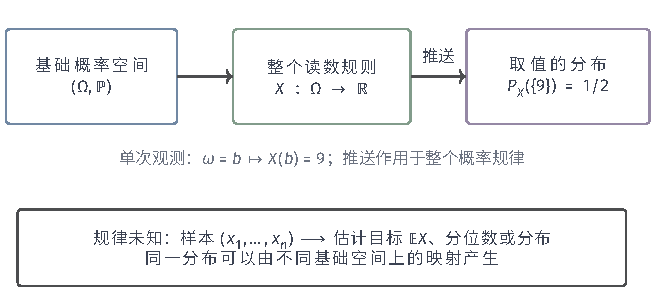
\includegraphics[width=\linewidth]{figures/01-mathematical-preliminaries/04-random-variables-distributions-and-causality/tikz/rv-objects/figure.pdf}
  \caption{基础结果经随机变量映射成为读数；把事件概率推送到取值空间得到分布。分布未知时，样本用于估计指定目标，并不能唯一还原基础空间上的映射。}
\label{fig:rv-objects}
\end{figure}

% v1-probability-density-cdf tex/01-mathematical-preliminaries/04-random-variables-distributions-and-causality/01-random-variables.tex
\begin{figure*}[htbp]
  \centering
  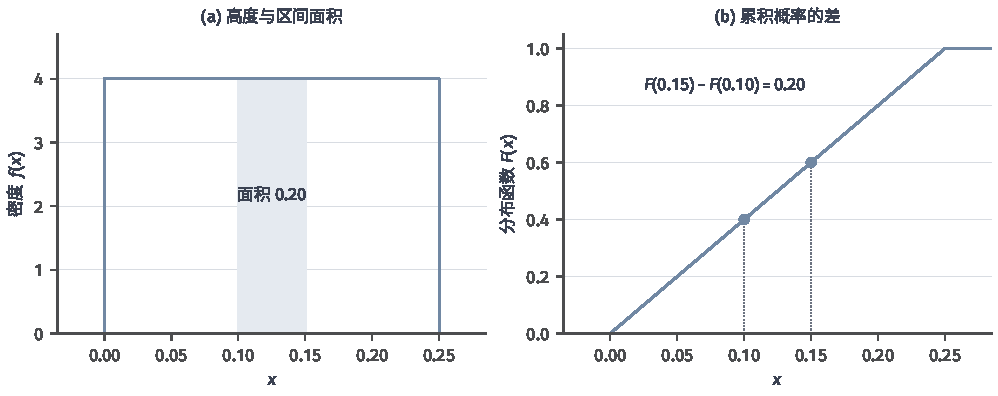
\includegraphics[width=\linewidth]{figures/01-mathematical-preliminaries/04-random-variables-distributions-and-causality/matplotlib/probability-density-cdf/figure.pdf}
  \caption{区间\([0,1/4]\)上的均匀分布（解析式教学图）。左图阴影为\([0.10,0.15]\)的概率\(0.20\)，密度高度为\(4\)；右图的概率是\(F(0.15)-F(0.10)\)，两个端点本身均没有正概率质量。}
  \label{fig:probability-density-cdf}
\end{figure*}

% v1-rv-paths tex/01-mathematical-preliminaries/04-random-variables-distributions-and-causality/01-random-variables.tex
\begin{figure}[htbp]
  \centering
  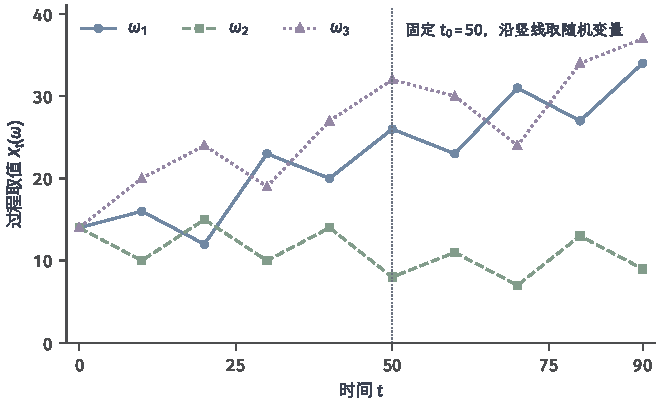
\includegraphics[width=\linewidth]{figures/01-mathematical-preliminaries/04-random-variables-distributions-and-causality/matplotlib/rv-paths/figure.pdf}
  \caption{同一过程的路径与时刻截面是不同对象。图为人为给定的三条示意路径，竖虚线固定时刻\(t_0\)；交点展示该时刻可能出现的不同值，并非用三条路径估计出的概率密度。}
\label{fig:rv-paths}
\end{figure}

% v1-rv-dependence tex/01-mathematical-preliminaries/04-random-variables-distributions-and-causality/01-random-variables.tex
\begin{figure}[htbp]
  \centering
  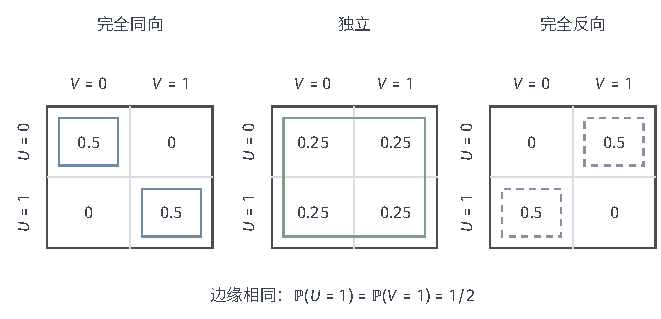
\includegraphics[width=\linewidth]{figures/01-mathematical-preliminaries/04-random-variables-distributions-and-causality/tikz/rv-dependence/figure.pdf}
  \caption{边缘质量相同的三个联合分布。格内数字是联合概率，各行各列的和始终为\(1/2\)；质量的位置改变协方差及和的分布。}
\label{fig:rv-dependence}
\end{figure}

% v1-probability-importance-weights tex/01-mathematical-preliminaries/04-random-variables-distributions-and-causality/01-random-variables.tex
\begin{figure*}[htbp]
  \centering
  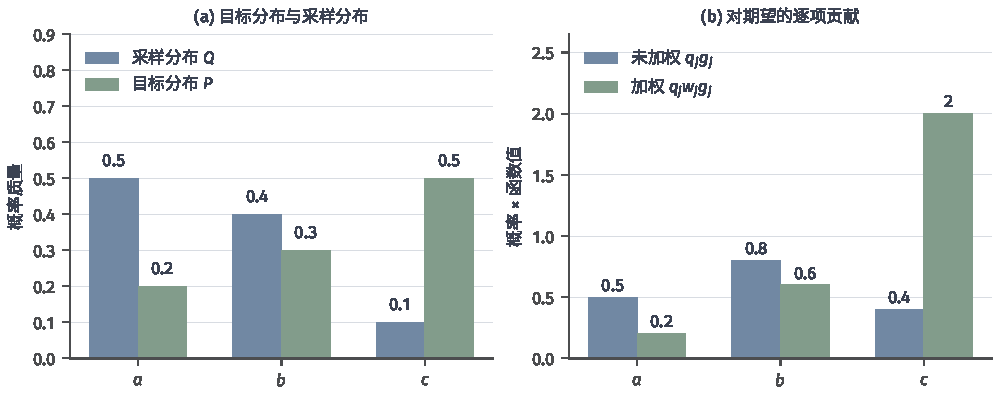
\includegraphics[width=\linewidth]{figures/01-mathematical-preliminaries/04-random-variables-distributions-and-causality/matplotlib/probability-importance-weights/figure.pdf}
  \caption{三结果换测度的有限构造。左图比较采样分布\(Q\)与目标分布\(P\)，右图比较\(q_jg_j\)与\(q_jw_jg_j=p_jg_j\)。各柱从零起画；右图柱高之和分别为\(1.7\)和\(2.8\)，并非单点概率。}
  \label{fig:probability-importance-weights}
\end{figure*}

% v1-rv-poisson-compensation tex/01-mathematical-preliminaries/04-random-variables-distributions-and-causality/01-random-variables.tex
\begin{figure}[htbp]
  \centering
  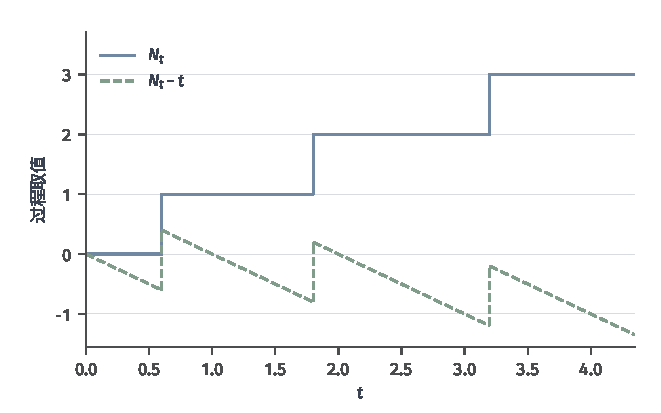
\includegraphics[width=\linewidth]{figures/01-mathematical-preliminaries/04-random-variables-distributions-and-causality/matplotlib/rv-poisson-compensation/figure.pdf}
  \caption{给定三次到达时刻的教学路径，取\(\lambda=1\)。蓝线为计数\(N_t\)，绿虚线为\(\widetilde N_t=N_t-t\)；两条路径在同一时刻跳跃且跳跃量相同。减去的是平均趋势，不是实现中的跳跃。}
\label{fig:rv-poisson-compensation}
\end{figure}

% v1-reader-brownian-quadratic-variation tex/01-mathematical-preliminaries/04-random-variables-distributions-and-causality/01-random-variables.tex
\begin{figure*}[htbp]
  \centering
  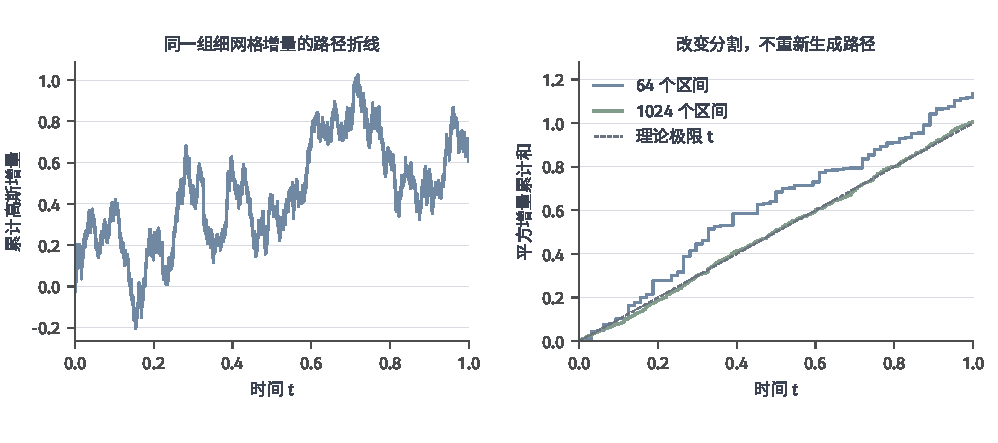
\includegraphics[width=\linewidth]{figures/01-mathematical-preliminaries/04-random-variables-distributions-and-causality/matplotlib/reader-brownian-quadratic-variation/figure.pdf}
  \caption{以固定随机种子构造的高斯增量教学例。左图由$4096$个独立增量
  $\Delta W_i\sim\mathcal N(0,1/4096)$累计成路径折线；右图将同一组增量分别合并为
  $64$和$1024$个时间区间，再累计各区间增量的平方。蓝、绿阶梯线使用不同分割，
  灰色参考线为理论二次变差$t$。这里只绘制有限网格，不把某一条折线作为连续布朗路径或收敛证明。}
  \label{fig:reader-brownian-quadratic-variation}
\end{figure*}

% v1-statistics-huber-loss tex/01-mathematical-preliminaries/04-random-variables-distributions-and-causality/01-random-variables.tex
\begin{figure*}[htbp]
  \centering
  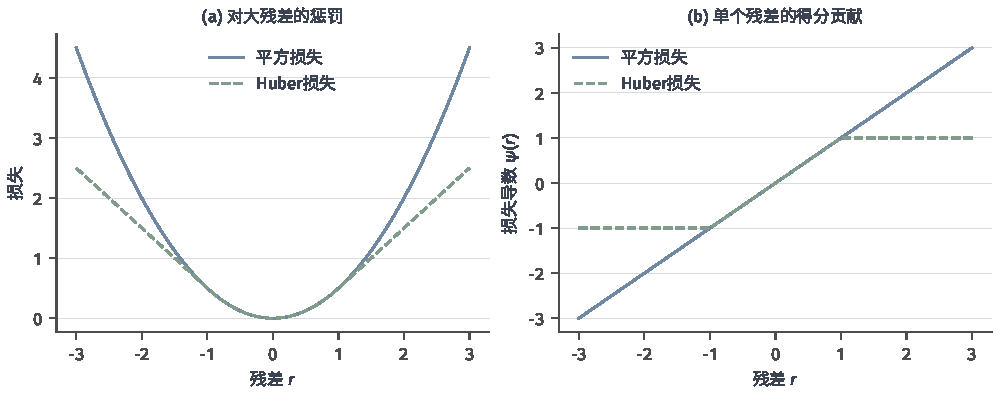
\includegraphics[width=\linewidth]{figures/01-mathematical-preliminaries/04-random-variables-distributions-and-causality/matplotlib/statistics-huber-loss/figure.pdf}
  \caption{平方损失与阈值\(c=1\)的Huber损失（解析式教学图）。左图比较惩罚值，右图比较对残差的导数；Huber得分在\([-1,1]\)内截断。横轴是构造残差，不代表实测异常值分布。}
  \label{fig:statistics-huber-loss}
\end{figure*}

% v1-statistics-local-boundary-fit tex/01-mathematical-preliminaries/04-random-variables-distributions-and-causality/01-random-variables.tex
\begin{figure}[htbp]
  \centering
  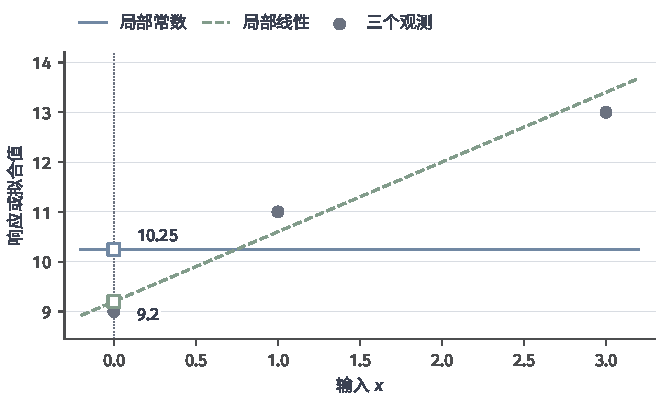
\includegraphics[width=\linewidth]{figures/01-mathematical-preliminaries/04-random-variables-distributions-and-causality/matplotlib/statistics-local-boundary-fit/figure.pdf}
  \caption{边界处的局部常数与局部线性拟合（教学数据图）。观测为\((0,9),(1,11),(3,13)\)，权重为\(1,0.75,0.25\)。蓝实线为加权常数\(10.25\)，绿虚线为\(9.2+1.4x\)，边界\(x_0=0\)处分别预测\(10.25\)和\(9.2\)。}
  \label{fig:statistics-local-boundary-fit}
\end{figure}

% v1-statistics-mean-prediction-width tex/01-mathematical-preliminaries/04-random-variables-distributions-and-causality/01-random-variables.tex
\begin{figure}[htbp]
  \centering
  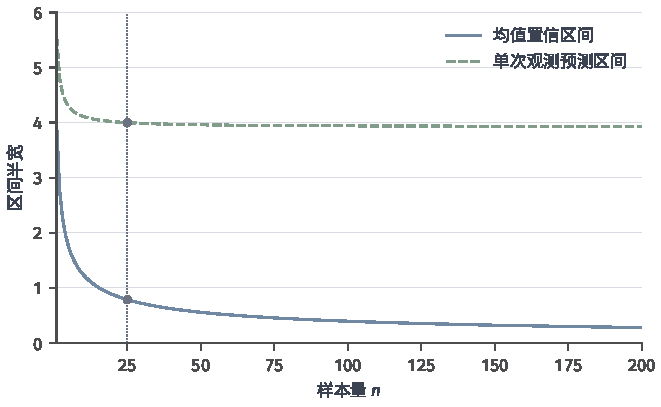
\includegraphics[width=\linewidth]{figures/01-mathematical-preliminaries/04-random-variables-distributions-and-causality/matplotlib/statistics-mean-prediction-width/figure.pdf}
  \caption{已知\(\sigma=2\)的独立高斯位置模型中，两类区间半宽随样本量变化（解析式教学图）。使用四舍五入分位数\(1.96\)，蓝实线为\(1.96\sigma/\sqrt n\)，绿虚线为\(1.96\sigma\sqrt{1+1/n}\)。灰竖线标出例~\ref{ex:statistics-running-sensor-calibration}的\(n=25\)，没有对任何实测数据重复抽样。}
  \label{fig:statistics-mean-prediction-width}
\end{figure}

% v1-stochastic-design-ellipsoids tex/01-mathematical-preliminaries/04-random-variables-distributions-and-causality/01-random-variables.tex
\begin{figure}[htbp]
  \centering
  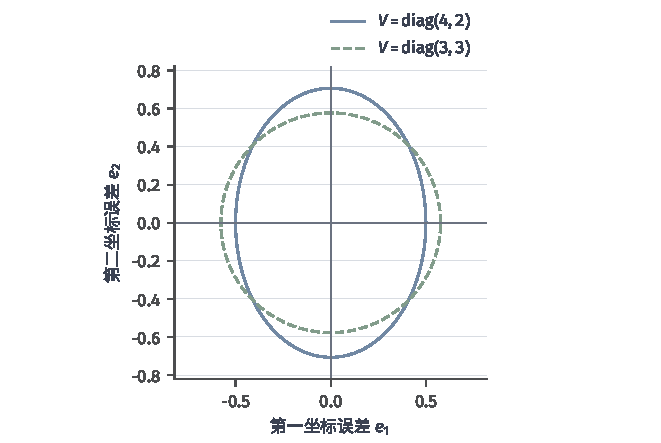
\includegraphics[width=\linewidth]{figures/01-mathematical-preliminaries/04-random-variables-distributions-and-causality/matplotlib/stochastic-design-ellipsoids/figure.pdf}
  \caption{二维设计的归一化误差几何（解析式教学图）。蓝实线为\(\bm e^\top\operatorname{diag}(4,2)\bm e=1\)，绿虚线为\(\bm e^\top\operatorname{diag}(3,3)\bm e=1\)。它们不是已经具有相同覆盖概率的数值置信区间；真实置信半径由式~\eqref{eq:stoch-adaptive-confidence-ellipsoid}另行确定。}
  \label{fig:stochastic-design-ellipsoids}
\end{figure}

% v1-probability-vanishing-spikes tex/01-mathematical-preliminaries/04-random-variables-distributions-and-causality/01-random-variables.tex
\begin{figure*}[htbp]
  \centering
  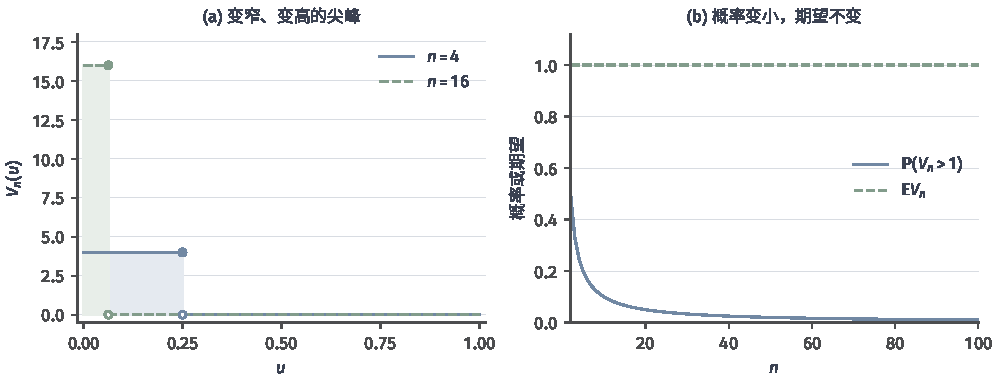
\includegraphics[width=\linewidth]{figures/01-mathematical-preliminaries/04-random-variables-distributions-and-causality/matplotlib/probability-vanishing-spikes/figure.pdf}
  \caption{小概率尖峰与期望质量（解析式教学图）。左图为\(V_n(u)=n\mathbb I\{u\leq1/n\}\)在\(n=4,16\)时的取值，均以面积\(1\)贡献期望；右图对\(n\geq2\)显示\(\mathbb P(V_n>1)=1/n\)趋于零，而\(\mathbb E V_n=1\)不变。基础变量为\(U\sim\operatorname{Unif}(0,1)\)。}
  \label{fig:probability-vanishing-spikes}
\end{figure*}

% v1-stochastic-mixing-variance tex/01-mathematical-preliminaries/04-random-variables-distributions-and-causality/01-random-variables.tex
\begin{figure*}[htbp]
  \centering
  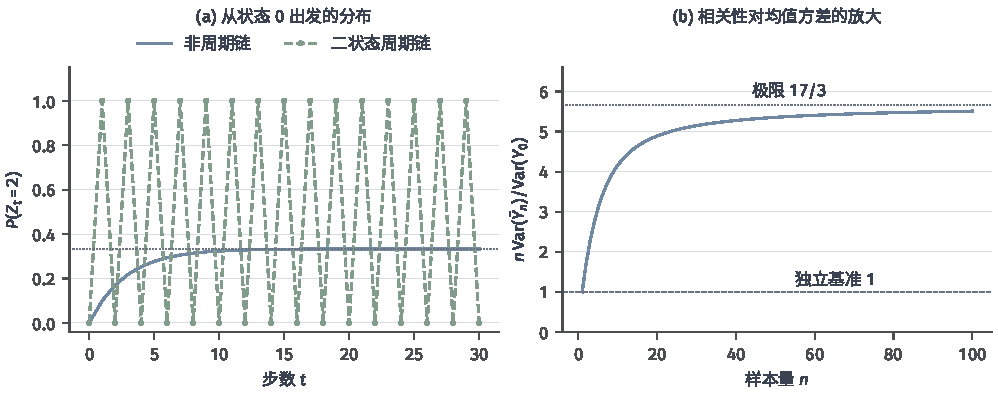
\includegraphics[width=\linewidth]{figures/01-mathematical-preliminaries/04-random-variables-distributions-and-causality/matplotlib/stochastic-mixing-variance/figure.pdf}
  \caption{两状态链的解析式教学图。左图蓝线使用例~\ref{ex:stoch-two-state-chain}的转移矩阵，从\(Z_0=0\)出发绘制\(\mathbb P(Z_t=2)=(1-0.7^t)/3\)；绿线使用确定交替的转移矩阵。右图使用平稳初态和\(\rho_k=0.7^k\)，绘制\(1+2\sum_{k=1}^{n-1}(1-k/n)\rho_k\)，其极限为\(17/3\)，独立观测基准为\(1\)。}
  \label{fig:stochastic-mixing-variance}
\end{figure*}

% v1-information-kernel-distinguishability tex/01-mathematical-preliminaries/04-random-variables-distributions-and-causality/02-information-theory-and-statistical-geometry.tex
\begin{figure*}[htbp]
  \centering
  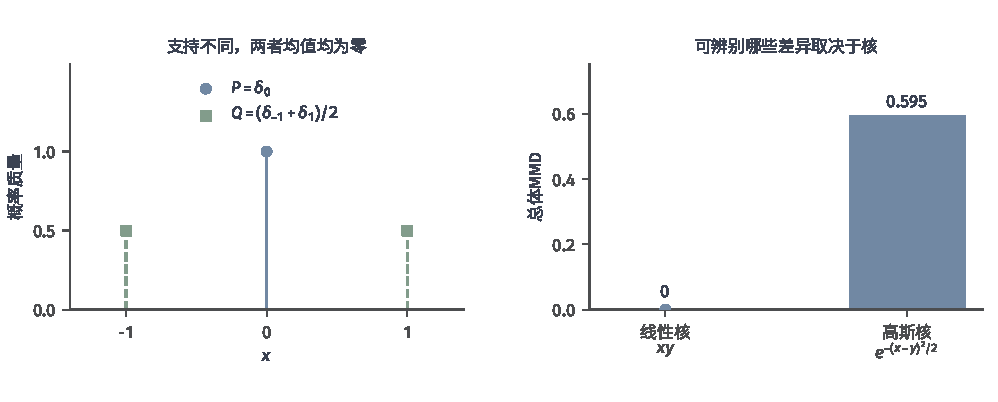
\includegraphics[width=\linewidth]{figures/01-mathematical-preliminaries/04-random-variables-distributions-and-causality/matplotlib/information-kernel-distinguishability/figure.pdf}
  \caption{同均值分布在不同核下的MMD（解析式教学图）。左图为\(P=\delta_0\)与\(Q=(\delta_{-1}+\delta_1)/2\)，右图按精确总体期望计算：线性核给出零，高斯核给出约\(0.595\)。没有使用有限样本估计；差别来自测试函数类。}
  \label{fig:information-kernel-distinguishability}
\end{figure*}

% v1-information-gaussian-distances tex/01-mathematical-preliminaries/04-random-variables-distributions-and-causality/02-information-theory-and-statistical-geometry.tex
\begin{figure*}[htbp]
  \centering
  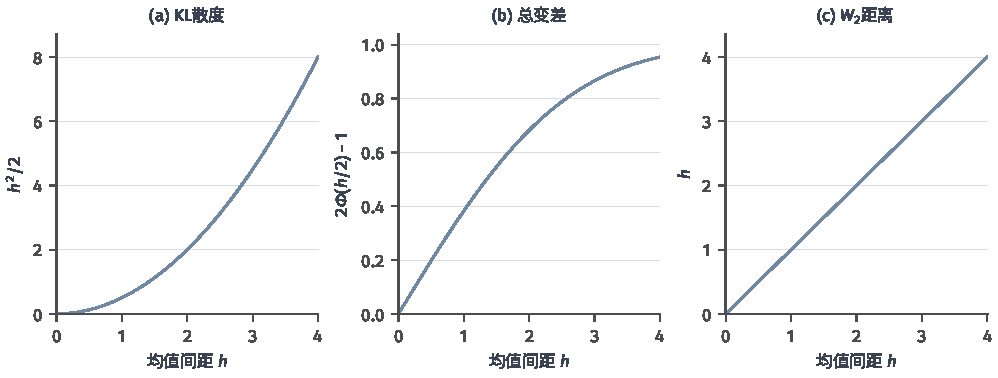
\includegraphics[width=\linewidth]{figures/01-mathematical-preliminaries/04-random-variables-distributions-and-causality/matplotlib/information-gaussian-distances/figure.pdf}
  \caption{同方差高斯位置族的解析式比较。固定\(P=\mathcal N(0,1)\)、\(Q=\mathcal N(h,1)\)，三图分别为\(D_{\mathrm{KL}}=h^2/2\)、\(d_{\mathrm{TV}}=2\Phi(h/2)-1\)与\(W_2=h\)，图中\(h\geq0\)。纵轴分别表达对数代价、事件概率差与搬运位移。}
  \label{fig:information-gaussian-distances}
\end{figure*}

% v1-information-binary-channel-information tex/01-mathematical-preliminaries/04-random-variables-distributions-and-causality/02-information-theory-and-statistical-geometry.tex
\begin{figure}[htbp]
  \centering
  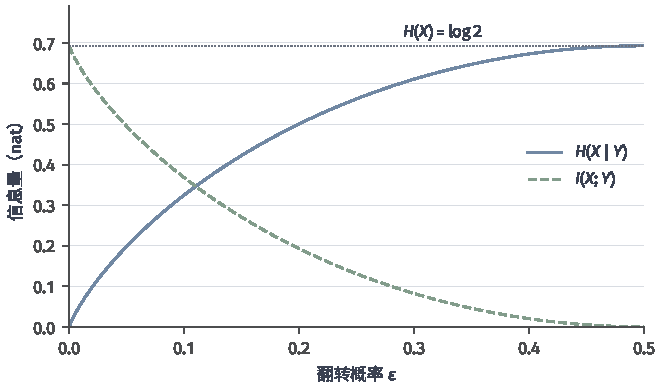
\includegraphics[width=\linewidth]{figures/01-mathematical-preliminaries/04-random-variables-distributions-and-causality/matplotlib/information-binary-channel-information/figure.pdf}
  \caption{公平二元输入通过独立翻转通道后的信息分配（解析式教学图）。蓝实线为剩余条件熵\(H_{\mathrm b}(\varepsilon)\)，绿虚线为互信息\(\log2-H_{\mathrm b}(\varepsilon)\)，均以nat计。输入熵保持不变，零噪声与公平翻转分别对应完整信息与零信息。}
  \label{fig:information-binary-channel-information}
\end{figure}

% v1-information-small-shift-task tex/01-mathematical-preliminaries/04-random-variables-distributions-and-causality/02-information-theory-and-statistical-geometry.tex
\begin{figure}[htbp]
  \centering
  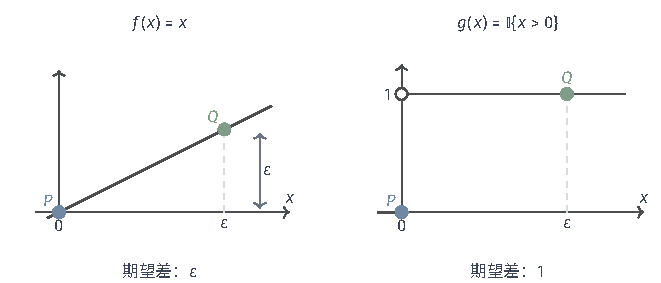
\includegraphics[width=\linewidth]{figures/01-mathematical-preliminaries/04-random-variables-distributions-and-causality/tikz/information-small-shift-task/figure.pdf}
  \caption{同一小位移对两种固定评价的影响。取\(P=\delta_0\)、
  \(Q=\delta_\varepsilon\)、\(\varepsilon>0\)，底层距离为绝对值。
  左图的\(1\)-Lipschitz函数\(f(x)=x\)变化\(\varepsilon\)；
  右图的事件函数\(\mathbb I\{x>0\}\)变化\(1\)。横向位置仅作示意，
  结论对任意正的\(\varepsilon\)成立。}
  \label{fig:information-small-shift-task}
\end{figure}

% v1-information-transport-tables tex/01-mathematical-preliminaries/04-random-variables-distributions-and-causality/02-information-theory-and-statistical-geometry.tex
\begin{figure}[htbp]
  \centering
  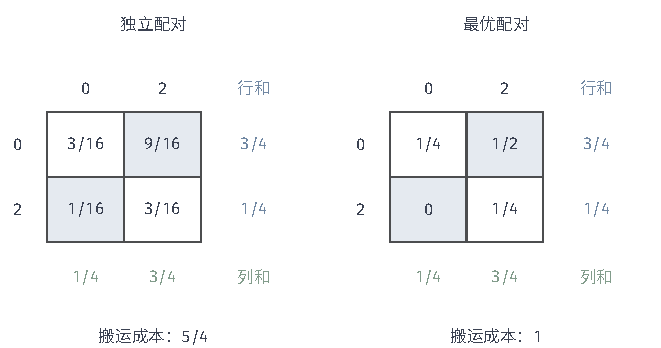
\includegraphics[width=\linewidth]{figures/01-mathematical-preliminaries/04-random-variables-distributions-and-causality/tikz/information-transport-tables/figure.pdf}
  \caption{同一边缘约束下的两张搬运表。来源和目标都位于\(0,2\)，
  蓝色行和为\(\bm p=(3/4,1/4)\)，绿色列和为\(\bm q=(1/4,3/4)\)。
  浅色单元格承担非零距离成本。独立表的成本为\(5/4\)，最优表为\(1\)；
  正文的势函数给出与最优表相等的对偶值。}
  \label{fig:information-transport-tables}
\end{figure}

% v1-information-fisher-local tex/01-mathematical-preliminaries/04-random-variables-distributions-and-causality/02-information-theory-and-statistical-geometry.tex
\begin{figure*}[htbp]
  \centering
  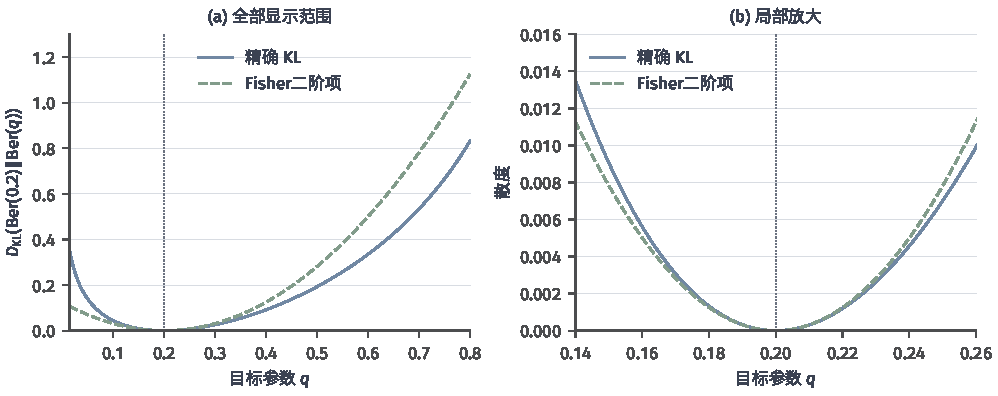
\includegraphics[width=\linewidth]{figures/01-mathematical-preliminaries/04-random-variables-distributions-and-causality/matplotlib/information-fisher-local/figure.pdf}
  \caption{Bernoulli族在\(p=0.2\)处的Fisher局部近似（解析式教学图）。
  蓝实线为\(D_{\mathrm{KL}}(P_{0.2}\Vert P_q)\)，绿虚线为
  \((q-0.2)^2/[2(0.2)(0.8)]\)；右图放大邻域。图中\(0<q<1\)，
  二阶式只描述足够小的参数扰动。}
  \label{fig:information-fisher-local}
\end{figure*}

% v1-information-natural-gradient-ellipse tex/01-mathematical-preliminaries/04-random-variables-distributions-and-causality/02-information-theory-and-statistical-geometry.tex
\begin{figure}[htbp]
  \centering
  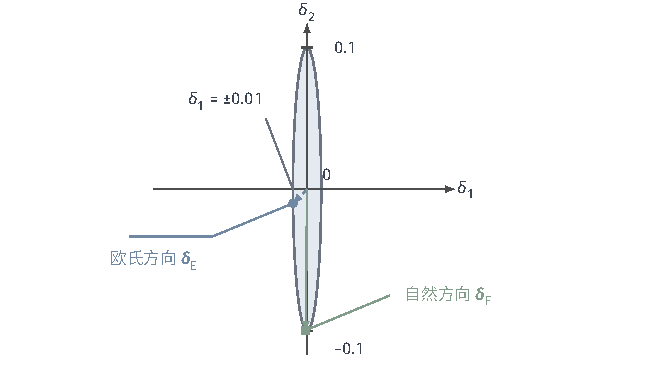
\includegraphics[width=\linewidth]{figures/01-mathematical-preliminaries/04-random-variables-distributions-and-causality/tikz/information-natural-gradient-ellipse/figure.pdf}
  \caption{局部KL预算下的下降方向（解析式教学图）。灰色椭圆满足
  \(100\delta_1^2+\delta_2^2=0.01\)，对应\(\varepsilon=0.005\)。
  蓝色虚线与圆点是缩放后的欧氏方向\(\bm\delta_{\mathrm E}\)，绿色实线与方点是
  自然方向\(\bm\delta_{\mathrm F}\)；两个终点消耗相同的二次预算。
  椭圆表达分布变化代价，不是目标函数的等高线。}
  \label{fig:information-natural-gradient-ellipse}
\end{figure}

% v1-causal-cross-world-couplings tex/01-mathematical-preliminaries/04-random-variables-distributions-and-causality/03-causal-response-and-structure.tex
\begin{figure}[htbp]
  \centering
  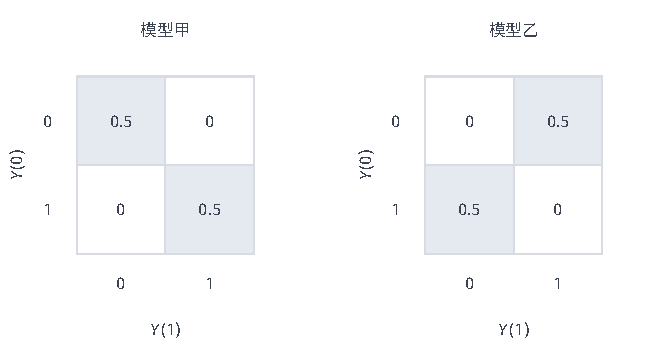
\includegraphics[width=\linewidth]{figures/01-mathematical-preliminaries/04-random-variables-distributions-and-causality/tikz/causal-cross-world-couplings/figure.pdf}
  \caption{相同干预边缘的两种跨世界配对。行对应\(Y(0)\)，列对应\(Y(1)\)，格内
  数字为联合概率；每张表的行和、列和均为\(1/2\)。甲的个体效应恒为零，乙的个体
  效应等概率取\(1,-1\)，两者ATE均为零。这是相容机制的教学构造，不是随机试验
  直接观察到的潜在结果联合表。}
  \label{fig:causal-cross-world-couplings}
\end{figure}

% v1-causal-confounding-coverage tex/01-mathematical-preliminaries/04-random-variables-distributions-and-causality/03-causal-response-and-structure.tex
\begin{figure*}[htbp]
  \centering
  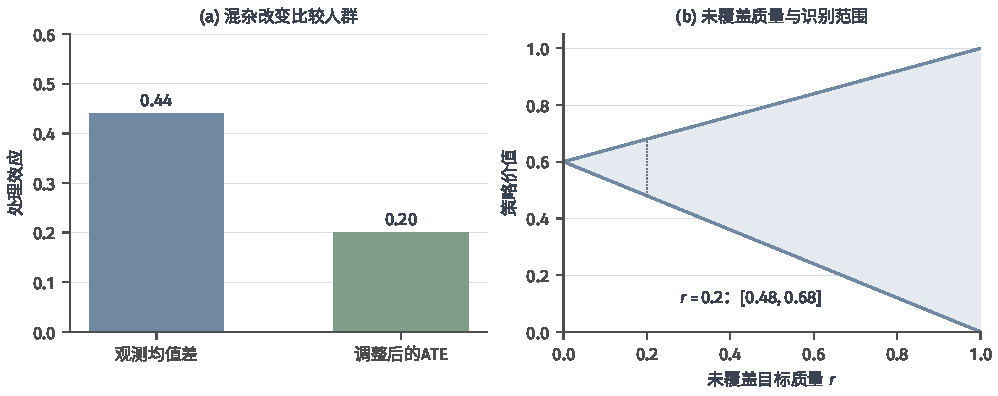
\includegraphics[width=\linewidth]{figures/01-mathematical-preliminaries/04-random-variables-distributions-and-causality/matplotlib/causal-confounding-coverage/figure.pdf}
  \caption{两个独立的教学构造。左图比较风险分层例子的观测均值差\(0.44\)与调整
  效应\(0.20\)。右图按式~\eqref{eq:causal-policy-value-bounds}绘制
  \([0.6(1-r),0.6(1-r)+r]\)。阴影为总体识别范围，不是抽样置信带；
  两个面板不表示同一数据集。}
  \label{fig:causal-confounding-coverage}
\end{figure*}

% v1-causal-local-path-patterns tex/01-mathematical-preliminaries/04-random-variables-distributions-and-causality/03-causal-response-and-structure.tex
\begin{figure*}[htbp]
  \centering
  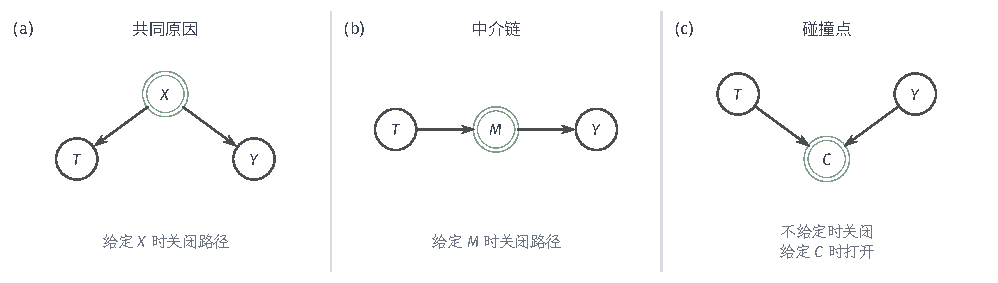
\includegraphics[width=\linewidth]{figures/01-mathematical-preliminaries/04-random-variables-distributions-and-causality/tikz/causal-local-path-patterns/figure.pdf}
  \caption{共同原因、中介与碰撞点的局部路径。双边框表示节点已加入条件集。
  共同原因和中介是非碰撞点，给定后关闭这条路径；给定碰撞点则打开原本关闭的
  路径。路径打开表示图不再保证相应独立性，并不指定相关的大小或正负。}
  \label{fig:causal-local-path-patterns}
\end{figure*}

% v1-causal-d-separation-paths tex/01-mathematical-preliminaries/04-random-variables-distributions-and-causality/03-causal-response-and-structure.tex
\begin{figure}[htbp]
  \centering
  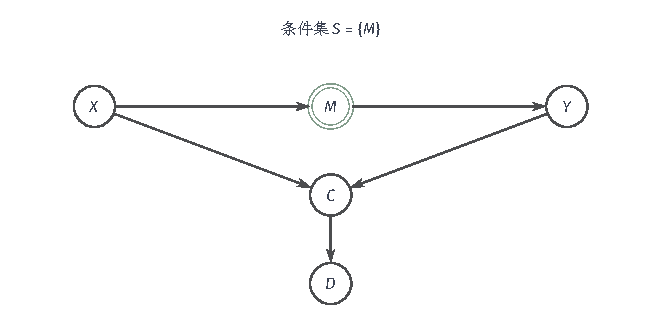
\includegraphics[width=\linewidth]{figures/01-mathematical-preliminaries/04-random-variables-distributions-and-causality/tikz/causal-d-separation-paths/figure.pdf}
  \caption{多条路径下的d-分离。双边框节点\(M\)属于条件集，上方链式路径关闭；
  碰撞点\(C\)及其后代\(D\)都未给定，下方路径也关闭。若再把\(C\)或\(D\)
  加入条件集，下方路径就会打开，说明增加条件可能破坏原有的分离。}
  \label{fig:causal-d-separation-paths}
\end{figure}

% v1-action-state-temperature-layers tex/01-mathematical-preliminaries/05-dynamical-systems-control-decision-and-games/01-action-and-state.tex
\begin{figure*}[htbp]
  \centering
  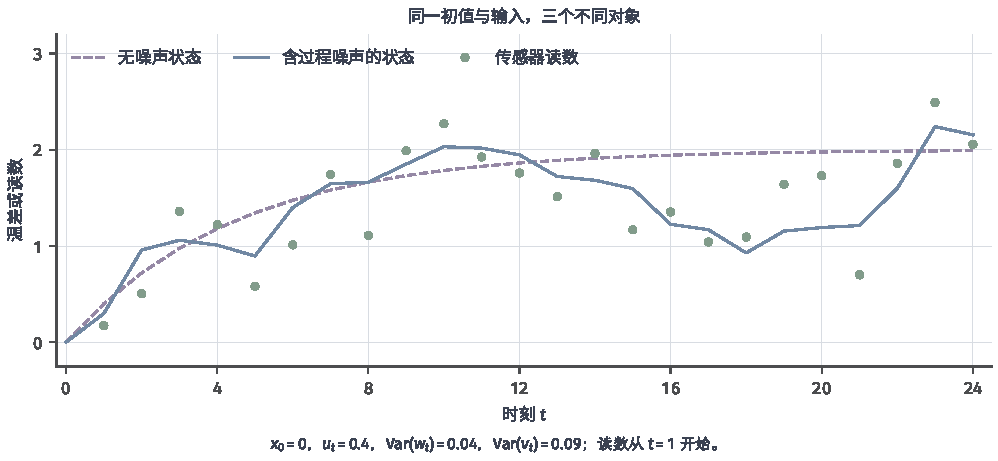
\includegraphics[width=\linewidth]{figures/01-mathematical-preliminaries/05-dynamical-systems-control-decision-and-games/matplotlib/action-state-temperature-layers/figure.pdf}
  \caption{同一温度模型的三个对象。初态$x_0=0$，输入始终为$0.4$；
  无噪声轨迹趋于$2$，过程噪声改变真实状态，独立观测噪声又把真实状态变成带噪读数。
  噪声方差分别为$0.04$和$0.09$。图中带噪曲线是固定种子的教学模拟，
  不是置信区间，也没有把读数用于反向校正状态。}
  \label{fig:action-state-temperature-layers}
\end{figure*}

% v1-action-state-ou-paths tex/01-mathematical-preliminaries/05-dynamical-systems-control-decision-and-games/01-action-and-state.tex
\begin{figure*}[htbp]
  \centering
  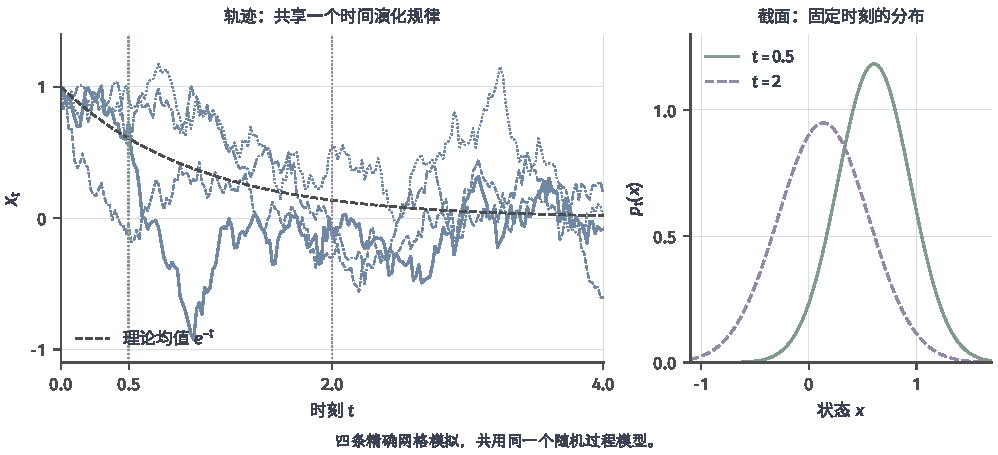
\includegraphics[width=\linewidth]{figures/01-mathematical-preliminaries/05-dynamical-systems-control-decision-and-games/matplotlib/action-state-ou-paths/figure.pdf}
  \caption{OU模型的路径与截面。取$\lambda=1,\sigma=0.6,X_0=1$，
 左侧为按精确高斯转移生成的四条网格轨迹与理论均值，右侧为$t=0.5,2$
 的解析边缘密度。折线只连接模拟网格点，不是可微的连续样本路径。
 截面给出单时刻概率，时间间的相关性还由共同噪声与转移决定。}
 \label{fig:action-state-ou-paths}
\end{figure*}

% v1-dynamical-euler-stability tex/01-mathematical-preliminaries/05-dynamical-systems-control-decision-and-games/01-action-and-state.tex
\begin{figure*}[htbp]
  \centering
  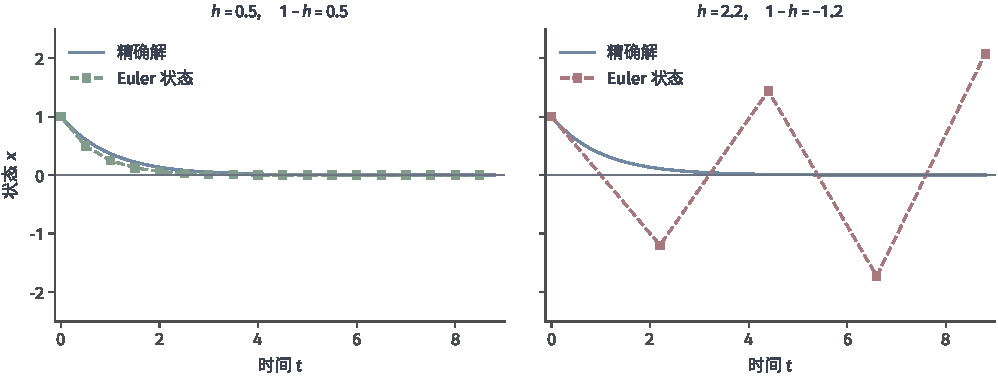
\includegraphics[width=\linewidth]{figures/01-mathematical-preliminaries/05-dynamical-systems-control-decision-and-games/matplotlib/dynamical-euler-stability/figure.pdf}
  \caption{教学方程$\dot x=-x$、$x(0)=1$的精确解与Euler近似。蓝色实线为精确解，
  方点为数值状态；左图绿色方点使用$h=0.5$并衰减，右图红色方点使用$h=2.2$并交替增长。两图采用相同坐标
  范围，连线只连接相邻数值状态。右图的发散来自步长，并非原连续系统不稳定。}
  \label{fig:dynamical-euler-stability}
\end{figure*}

% v1-reader-lasalle-zero-set tex/01-mathematical-preliminaries/05-dynamical-systems-control-decision-and-games/01-action-and-state.tex
\begin{figure}[htbp]
  \centering
  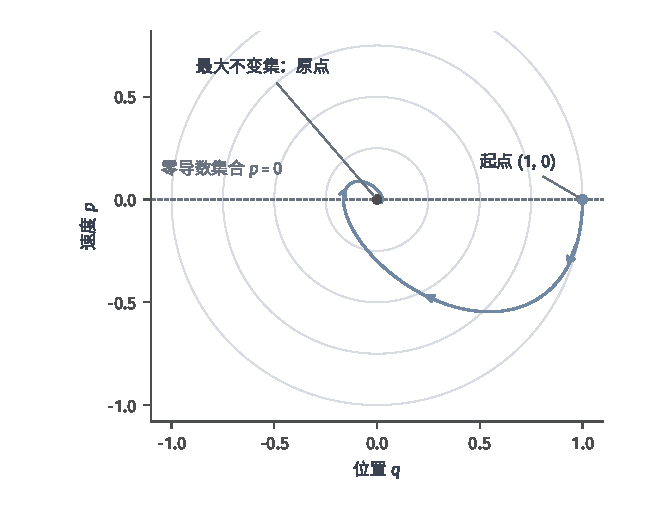
\includegraphics[width=\linewidth]{figures/01-mathematical-preliminaries/05-dynamical-systems-control-decision-and-games/matplotlib/reader-lasalle-zero-set/figure.pdf}
  \caption{阻尼振子$\dot q=p,\dot p=-q-p$从$(1,0)$出发的精确轨迹。
  蓝色轨迹覆盖$t=0$至$12$，箭头指示时间；灰色虚线为$\dot V=0$的直线$p=0$，
  浅灰圆为能量参考等值线。起点虽在零导数集合上，初始速度$(0,-1)$却将它带离
  该集合；能一直留在其中的完整轨迹只有原点。}
  \label{fig:reader-lasalle-zero-set}
\end{figure}

% v1-stochastic-stepsize-bias-variance tex/01-mathematical-preliminaries/05-dynamical-systems-control-decision-and-games/01-action-and-state.tex
\begin{figure*}[htbp]
  \centering
  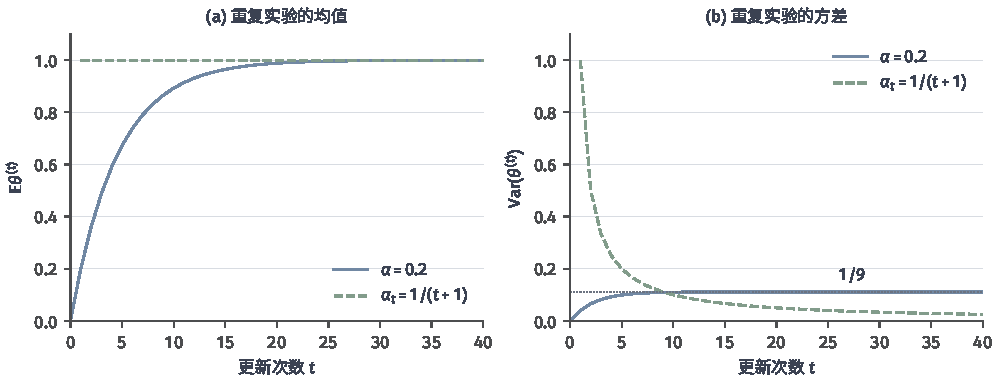
\includegraphics[width=\linewidth]{figures/01-mathematical-preliminaries/05-dynamical-systems-control-decision-and-games/matplotlib/stochastic-stepsize-bias-variance/figure.pdf}
  \caption{同一均值问题的重复实验均值与方差。取$\theta^{(0)}=0,\mu=1,\sigma^2=1$，
  观测独立同分布；蓝实线为固定$\alpha=0.2$，绿虚线为$\alpha_t=1/(t+1)$。
  固定步长方差趋于$1/9$，样本平均方差为$1/t$。曲线由解析式得到，不是一条样本轨迹。}
  \label{fig:stochastic-stepsize-bias-variance}
\end{figure*}

% v1-dynamical-transient-growth tex/01-mathematical-preliminaries/05-dynamical-systems-control-decision-and-games/01-action-and-state.tex
\begin{figure}[htbp]
  \centering
  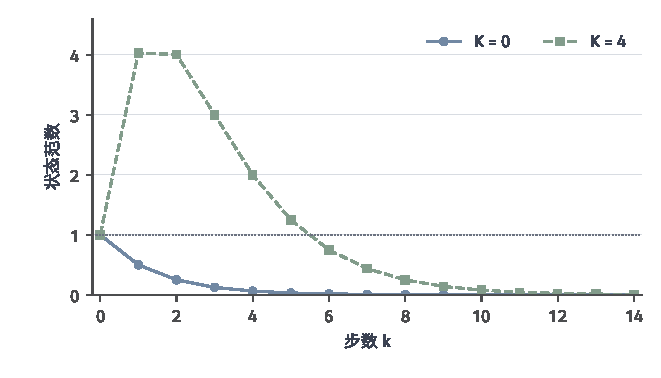
\includegraphics[width=\linewidth]{figures/01-mathematical-preliminaries/05-dynamical-systems-control-decision-and-games/matplotlib/dynamical-transient-growth/figure.pdf}
  \caption{同谱系统的不同瞬态。初值均为$(0,1)^\top$，蓝色圆点取$K=0$，
  绿色方点取$K=4$，谱半径均为$1/2$。后者前两步范数约为$4.03$、$4.01$，
  随后才趋零；灰线为初始范数$1$。长期衰减不等于每一步都收缩。}
  \label{fig:dynamical-transient-growth}
\end{figure}

% v1-dynamical-kalman-density-update tex/01-mathematical-preliminaries/05-dynamical-systems-control-decision-and-games/01-action-and-state.tex
\begin{figure}[htbp]
  \centering
  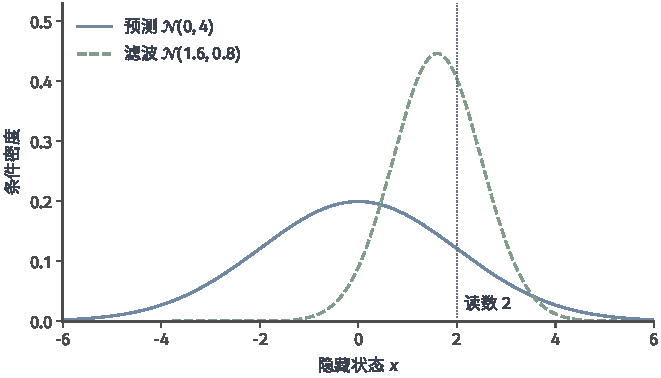
\includegraphics[width=\linewidth]{figures/01-mathematical-preliminaries/05-dynamical-systems-control-decision-and-games/matplotlib/dynamical-kalman-density-update/figure.pdf}
  \caption{独立标量教学例的预测$\mathcal N(0,4)$与后验$\mathcal N(1.6,0.8)$，
 实际读数$y=2$、观测噪声方差$1$。第二个高斯参数是方差；
 本图不是贯穿温度模型的参数设定。}
 \label{fig:dynamical-kalman-density-update}
\end{figure}

% v1-action-state-temperature-inference tex/01-mathematical-preliminaries/05-dynamical-systems-control-decision-and-games/01-action-and-state.tex
\begin{figure*}[htbp]
  \centering
  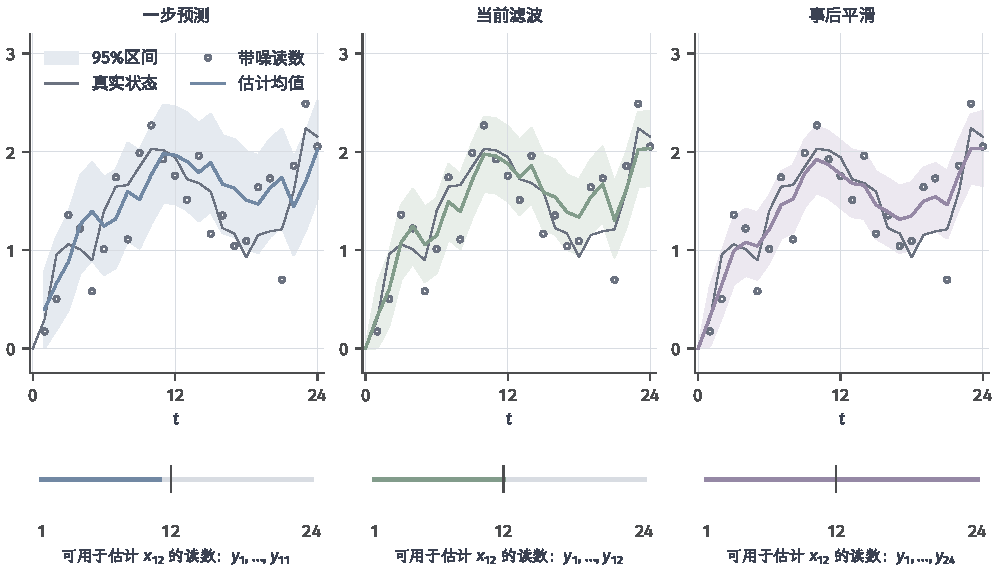
\includegraphics[width=\linewidth]{figures/01-mathematical-preliminaries/05-dynamical-systems-control-decision-and-games/matplotlib/action-state-temperature-inference/figure.pdf}
  \caption{与图~\ref{fig:action-state-temperature-layers}完全相同的温度轨迹及读数。
 三栏分别画一步预测、滤波与固定终点$T=24$的平滑均值和逐时刻$95\%$高斯区间，
 灰线为实际状态，圆点为读数；区间不是整条路径同时覆盖的置信带。
 下方以$t=12$为例标出可用观测范围。已知$x_0=0$，给定$u_t=0.4$，
 过程、观测方差仍为$0.04,0.09$。平滑的信息优势不是额外的在线能力。}
 \label{fig:action-state-temperature-inference}
\end{figure*}

% v1-control-reachable-directions tex/01-mathematical-preliminaries/05-dynamical-systems-control-decision-and-games/02-policy-realization-and-control.tex
\begin{figure}[htbp]
  \centering
  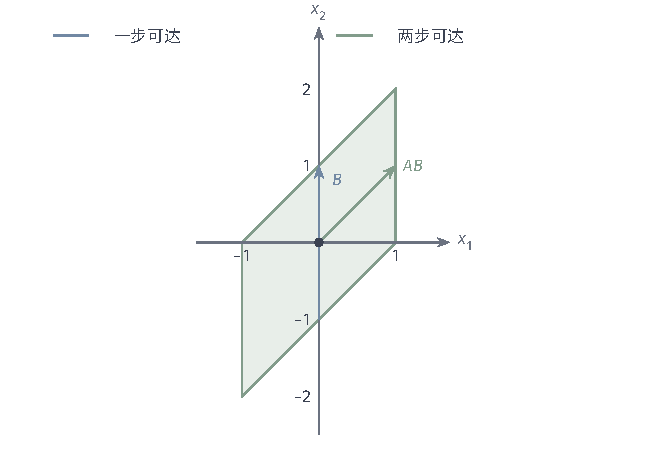
\includegraphics[width=\linewidth]{figures/01-mathematical-preliminaries/05-dynamical-systems-control-decision-and-games/tikz/control-reachable-directions/figure.pdf}
  \caption{教学系统$\bm A=\left[\begin{smallmatrix}1&1\\0&1\end{smallmatrix}\right]$、
  $\bm B=(0,1)^\top$从零出发。蓝色线段为$|u_0|\leq1$的一步可达集合，
  绿色区域为$|u_0|,|u_1|\leq1$的两步可达集合；箭头为$\bm B$与$\bm A\bm B$。
  幅值限制用于显示可达区域，不属于无约束可控性秩判据的假设。}
  \label{fig:control-reachable-directions}
\end{figure}

% v1-control-temperature-regulation-tracking tex/01-mathematical-preliminaries/05-dynamical-systems-control-decision-and-games/02-policy-realization-and-control.tex
\begin{figure*}[htbp]
  \centering
  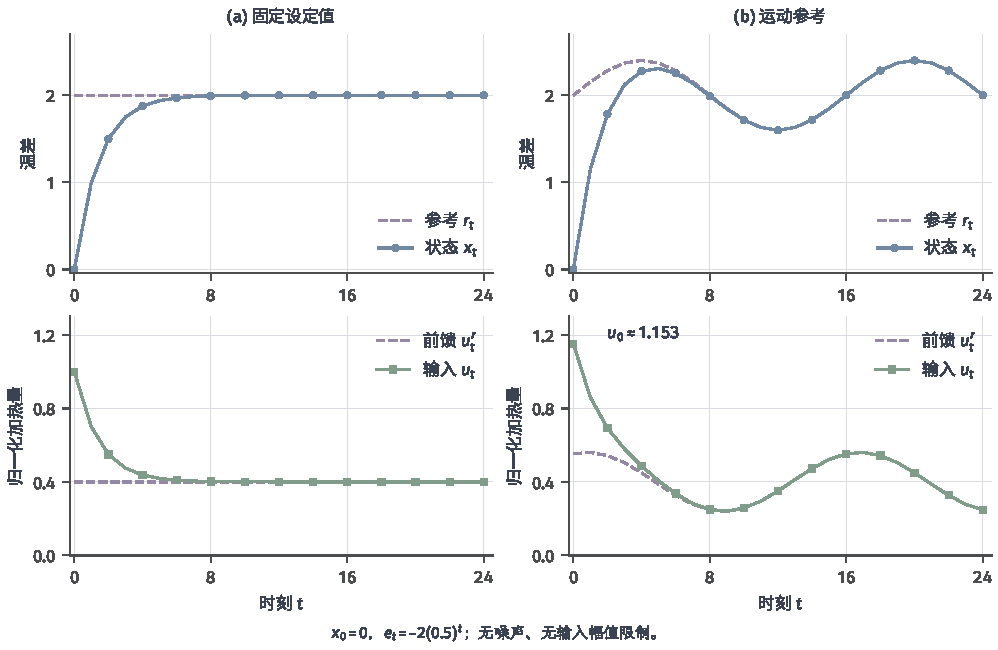
\includegraphics[width=\linewidth]{figures/01-mathematical-preliminaries/05-dynamical-systems-control-decision-and-games/matplotlib/control-temperature-regulation-tracking/figure.pdf}
  \caption{同一无噪声温度模型、初态$x_0=0$与误差增益$0.3$下的调节和跟踪。
  左列固定$r_t=2$，右列取$r_t=2+0.4\sin(\pi t/8)$；上排比较参考与实际状态，
  下排比较维持参考的前馈与完整输入。两种任务的误差均为$e_t=-2(0.5)^t$，
  但运动参考需要持续变化的前馈。图中输入无幅值限制，右下首个动作超过$1$，
  因而此图不是受限执行器的安全证明。离散点之间连线仅便于阅读。}
  \label{fig:control-temperature-regulation-tracking}
\end{figure*}

% v1-control-stability-safety tex/01-mathematical-preliminaries/05-dynamical-systems-control-decision-and-games/02-policy-realization-and-control.tex
\begin{figure}[htbp]
  \centering
  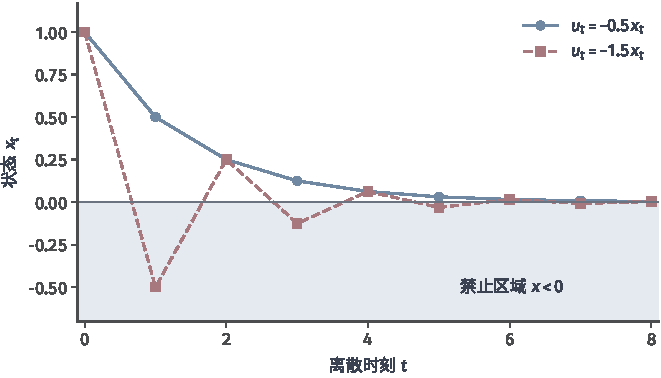
\includegraphics[width=\linewidth]{figures/01-mathematical-preliminaries/05-dynamical-systems-control-decision-and-games/matplotlib/control-stability-safety/figure.pdf}
  \caption{教学系统$x_{t+1}=x_t+u_t$从$x_0=1$出发。
  蓝色圆点采用$u_t=-0.5x_t$，保持$x_t\geq0$；
  红色方点采用$u_t=-1.5x_t$，第一步进入禁止的负半轴后交替衰减。
  两者都渐近稳定，只有前者保持安全集合。浅蓝区域表示禁止状态。}
  \label{fig:control-stability-safety}
\end{figure}

% v1-control-barrier-projection tex/01-mathematical-preliminaries/05-dynamical-systems-control-decision-and-games/02-policy-realization-and-control.tex
\begin{figure}[htbp]
  \centering
  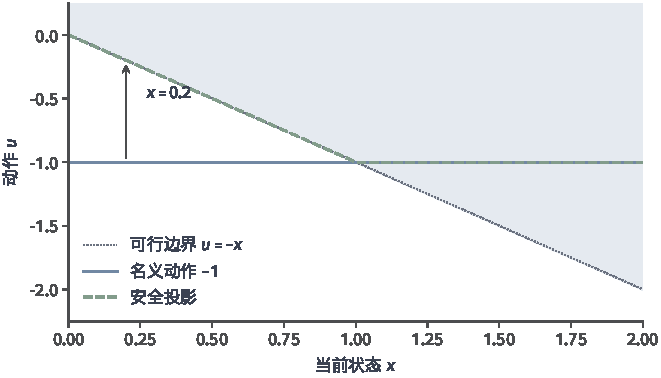
\includegraphics[width=\linewidth]{figures/01-mathematical-preliminaries/05-dynamical-systems-control-decision-and-games/matplotlib/control-barrier-projection/figure.pdf}
  \caption{教学积分器$\dot x_t=u_t$、安全集合$x\geq0$及$\alpha(h)=h$。
  灰色虚线$u=-x$上方为允许动作；蓝色实线为名义动作$u=-1$，
  绿色虚线为投影$u^\ast=\max\{-1,-x\}$。
  $x\geq1$处无需修正，$x=0.2$处修正为$-0.2$。
  图中没有额外执行器限制，不能据此判断有限输入范围下的联合可行性。}
  \label{fig:control-barrier-projection}
\end{figure}

% v1-decision-cvar-threshold tex/01-mathematical-preliminaries/05-dynamical-systems-control-decision-and-games/03-policy-value-and-optimization.tex
\begin{figure}[htbp]
  \centering
  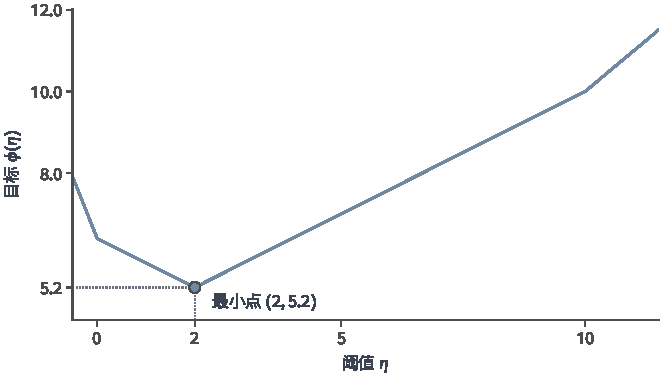
\includegraphics[width=\linewidth]{figures/01-mathematical-preliminaries/05-dynamical-systems-control-decision-and-games/matplotlib/decision-cvar-threshold/figure.pdf}
  \caption{教学分布$P(L=0)=0.6$、$P(L=2)=0.3$、$P(L=10)=0.1$在
  $\alpha=0.75$下的阈值目标$\phi(\eta)=\eta+4\mathbb E[(L-\eta)_+]$。
  蓝色折线的最小点为$(2,5.2)$；阈值$2$与尾部平均$5.2$不能混用。}
  \label{fig:decision-cvar-threshold}
\end{figure}

% v1-decision-cvar-reweighting tex/01-mathematical-preliminaries/05-dynamical-systems-control-decision-and-games/03-policy-value-and-optimization.tex
\begin{figure}[htbp]
  \centering
  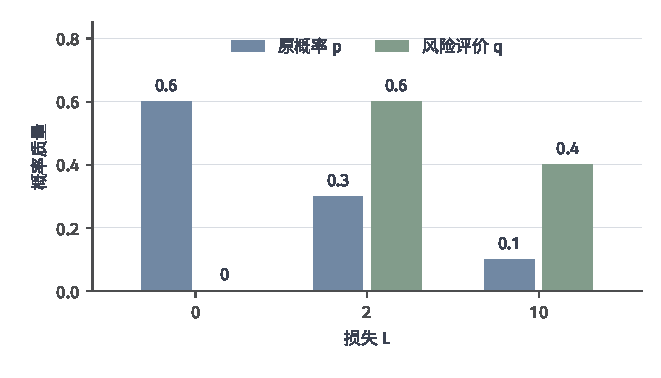
\includegraphics[width=\linewidth]{figures/01-mathematical-preliminaries/05-dynamical-systems-control-decision-and-games/matplotlib/decision-cvar-reweighting/figure.pdf}
  \caption{损失$0,2,10$的名义概率为$(0.6,0.3,0.1)$，CVaR$_{0.75}$的约束为
  $q_i\leq4p_i$和$\sum_iq_i=1$。最优重加权$(0,0.6,0.4)$的期望为$5.2$。
  蓝色为名义质量，绿色为对偶最优质量；真实发生概率并未因评价重加权而改变。}
  \label{fig:decision-cvar-reweighting}
\end{figure}

% v1-policy-temperature-comparison tex/01-mathematical-preliminaries/05-dynamical-systems-control-decision-and-games/03-policy-value-and-optimization.tex
\begin{figure*}[htbp]
  \centering
  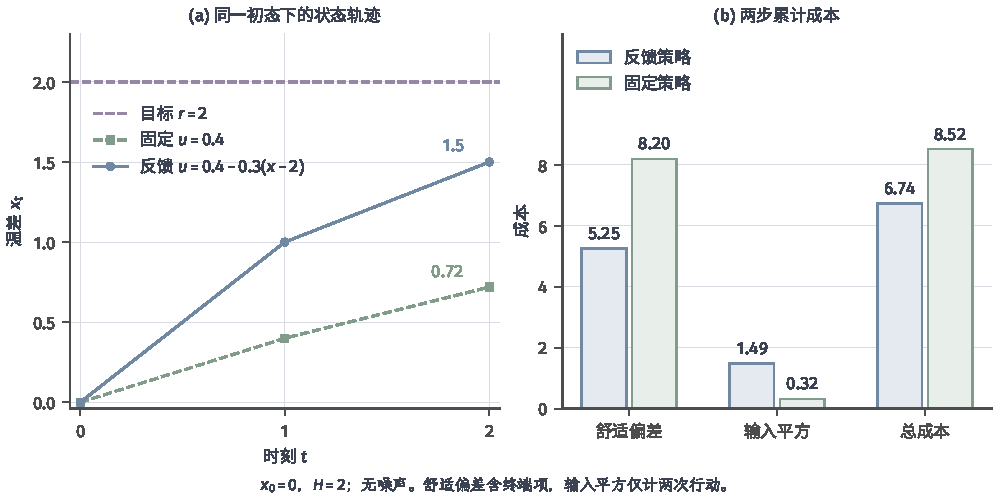
\includegraphics[width=\linewidth]{figures/01-mathematical-preliminaries/05-dynamical-systems-control-decision-and-games/matplotlib/policy-temperature-comparison/figure.pdf}
  \caption{共同温度模型下两项固定策略的比较。左图连接离散时刻的状态，紫色虚线为
  目标温差$2$；连线仅用于辨认轨迹，不表示额外的连续时间模型。右图按
  $c(x,u)=(x-2)^2+u^2$和终端成本$(x-2)^2$累计，柱顶数值保留两位小数。
  反馈的精确总成本为$6.74$，固定输入的总成本为$8.5184$。先分别求值再比较，
  并未在每一步重新选择最优行动。}
  \label{fig:policy-temperature-comparison}
\end{figure*}

% v1-decision-cost-thresholds tex/01-mathematical-preliminaries/05-dynamical-systems-control-decision-and-games/03-policy-value-and-optimization.tex
\begin{figure*}[htbp]
  \centering
  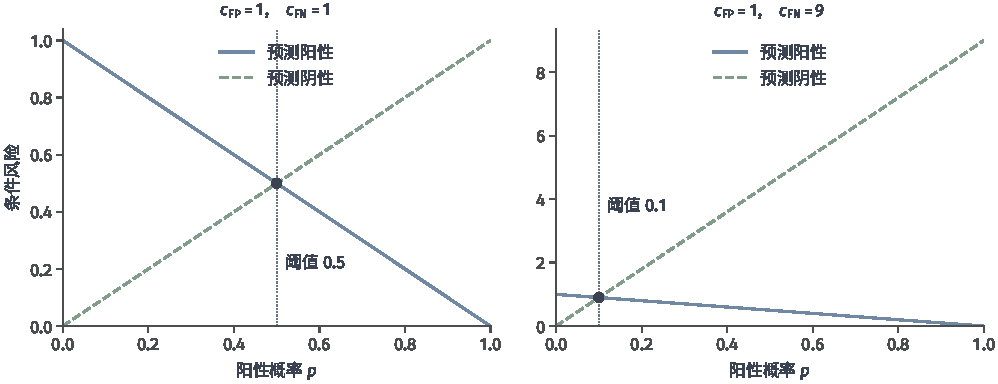
\includegraphics[width=\linewidth]{figures/01-mathematical-preliminaries/05-dynamical-systems-control-decision-and-games/matplotlib/decision-cost-thresholds/figure.pdf}
  \caption{二分类的条件风险。蓝色实线是预测阳性的$c_{\mathrm{FP}}(1-p)$，
  绿色虚线是预测阴性的$c_{\mathrm{FN}}p$。左图两种错误成本均为$1$，阈值$0.5$；
  右图漏诊成本增至$9$，阈值降为$0.1$。横轴相同，纵轴分别显示各自损失范围。}
  \label{fig:decision-cost-thresholds}
\end{figure*}

% v1-game-matching-best-responses tex/01-mathematical-preliminaries/05-dynamical-systems-control-decision-and-games/04-multi-agent-response-and-evolution.tex
\begin{figure}[htbp]
  \centering
  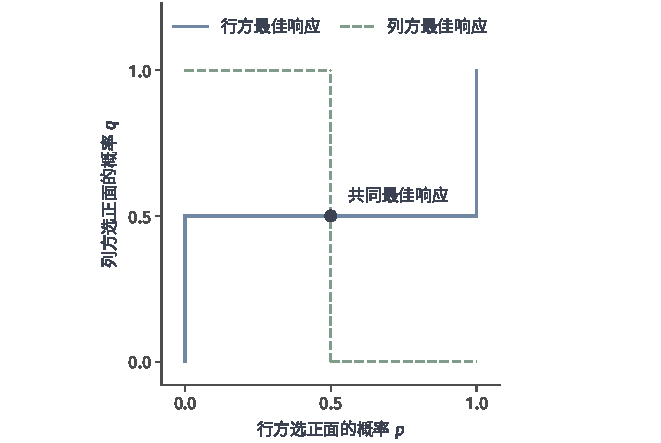
\includegraphics[width=\linewidth]{figures/01-mathematical-preliminaries/05-dynamical-systems-control-decision-and-games/matplotlib/game-matching-best-responses/figure.pdf}
  \caption{匹配硬币的最佳响应集合。横轴$p$、纵轴$q$分别是两方选$H$的概率。
  蓝色实线为行方响应，绿色虚线为列方响应；在$q=1/2$处行方允许全部$p$，
  在$p=1/2$处列方允许全部$q$，唯一共同点为$(1/2,1/2)$。
  这些线段描述允许的响应，不是实际运行的学习轨迹。}
  \label{fig:game-matching-best-responses}
\end{figure}

% v1-game-correlated-mass tex/01-mathematical-preliminaries/05-dynamical-systems-control-decision-and-games/04-multi-agent-response-and-evolution.tex
\begin{figure}[htbp]
  \centering
  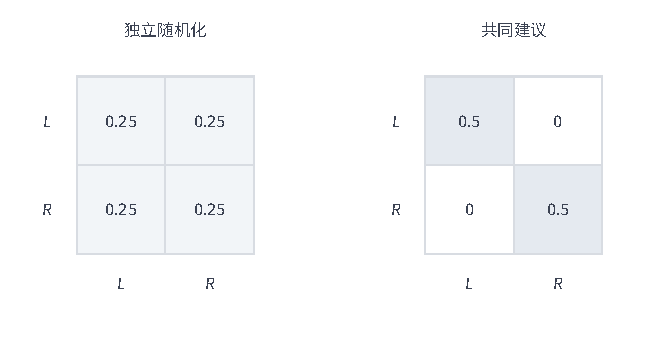
\includegraphics[width=\linewidth]{figures/01-mathematical-preliminaries/05-dynamical-systems-control-decision-and-games/tikz/game-correlated-mass/figure.pdf}
  \caption{二行动协调博弈的两个教学联合分布，共用$0$至$0.5$的概率色阶。
  行表示参与者1的行动，列表示参与者2的行动。左图为独立均匀策略，四格质量均为$0.25$；
  右图只推荐$(L,L)$与$(R,R)$，各占$0.5$。两者边缘概率均为$(0.5,0.5)$，
  但每人期望收益分别为$1$和$2$；相关分布并非边缘分布的乘积。}
  \label{fig:game-correlated-mass}
\end{figure}

% v1-game-bargaining-disagreement tex/01-mathematical-preliminaries/05-dynamical-systems-control-decision-and-games/04-multi-agent-response-and-evolution.tex
\begin{figure*}[htbp]
  \centering
  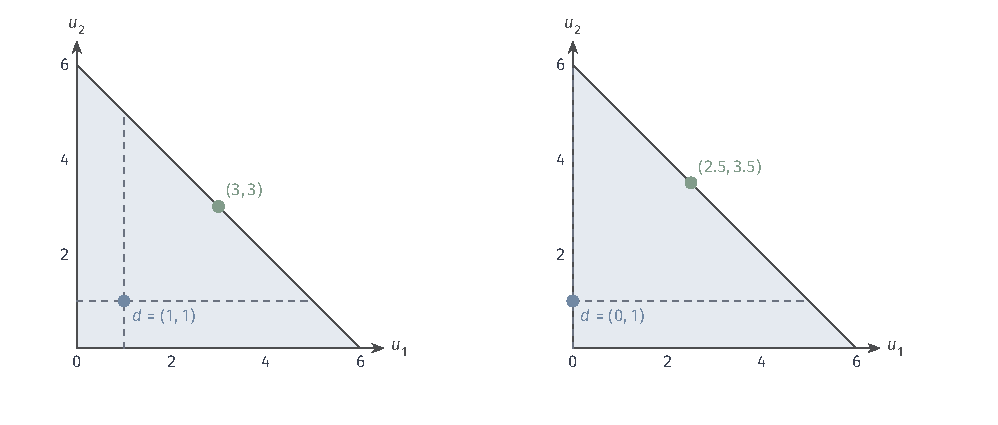
\includegraphics[width=\linewidth]{figures/01-mathematical-preliminaries/05-dynamical-systems-control-decision-and-games/tikz/game-bargaining-disagreement/figure.pdf}
  \caption{两方协商的教学可行域$u_1,u_2\geq0$、$u_1+u_2\leq6$，两图坐标一致。
  蓝点为分歧收益，绿点为相对该分歧点的Nash乘积最优解。左图$\bm d=(1,1)$得到
  $(3,3)$，右图$\bm d=(0,1)$得到$(2.5,3.5)$；灰色虚线给出个体可接受的下界。
  可行总收益没有变化，变化的是退出时可得到的收益。}
  \label{fig:game-bargaining-disagreement}
\end{figure*}

% v1-game-update-trajectories tex/01-mathematical-preliminaries/05-dynamical-systems-control-decision-and-games/04-multi-agent-response-and-evolution.tex
\begin{figure*}[htbp]
  \centering
  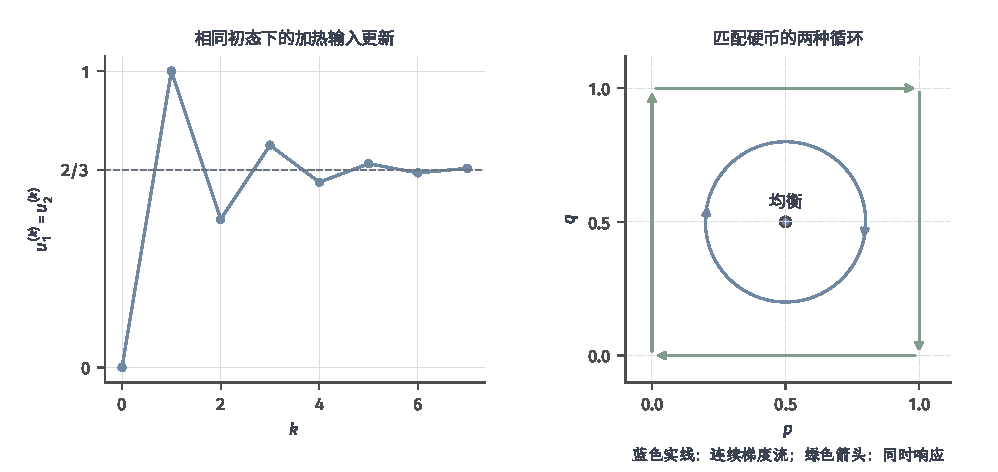
\includegraphics[width=\linewidth]{figures/01-mathematical-preliminaries/05-dynamical-systems-control-decision-and-games/matplotlib/game-update-trajectories/figure.pdf}
  \caption{两个已明确更新规则的教学轨迹。左图为相同初态下双加热器的同时最佳响应，
  从\(u_1^{(0)}=u_2^{(0)}=0\)开始，两条输入曲线重合，误差交替减半并趋向\(2/3\)。
  右图绿色方形箭头是匹配硬币的离散四周期，蓝色圆是内部连续梯度流从
  \((p,q)=(0.8,0.5)\)出发的闭轨道，中心标记是Nash均衡。
  圆与方形对应不同更新，均不是最佳响应对应图中的静态集合。}
  \label{fig:game-update-trajectories}
\end{figure*}

% v1-game-two-stage-self-reach tex/01-mathematical-preliminaries/05-dynamical-systems-control-decision-and-games/04-multi-agent-response-and-evolution.tex
\begin{figure}[htbp]
  \centering
  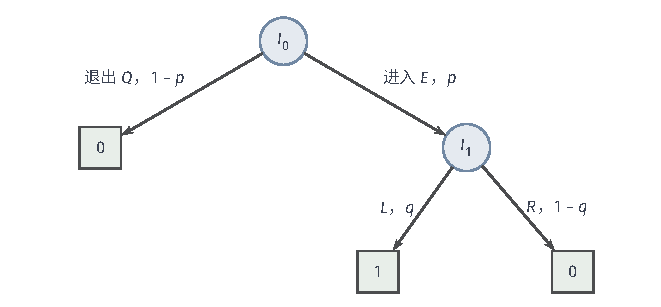
\includegraphics[width=\linewidth]{figures/01-mathematical-preliminaries/05-dynamical-systems-control-decision-and-games/tikz/game-two-stage-self-reach/figure.pdf}
  \caption{同一参与者$i$的两层决策。圆节点是其信息集，方节点中的数值是终局收益。
  第一步以概率$p$进入，第二步在已进入的条件下以概率$q$选$L$；
  因此到达收益为$1$的终局需经过两个本人行动，概率为$pq$。
  本图没有对手或机会节点，是用于区分自身到达概率与局部行动概率的教学构造。}
  \label{fig:game-two-stage-self-reach}
\end{figure}

% v1-decision-two-round-exploration tex/01-mathematical-preliminaries/05-dynamical-systems-control-decision-and-games/03-policy-value-and-optimization.tex
\begin{figure*}[htbp]
  \centering
  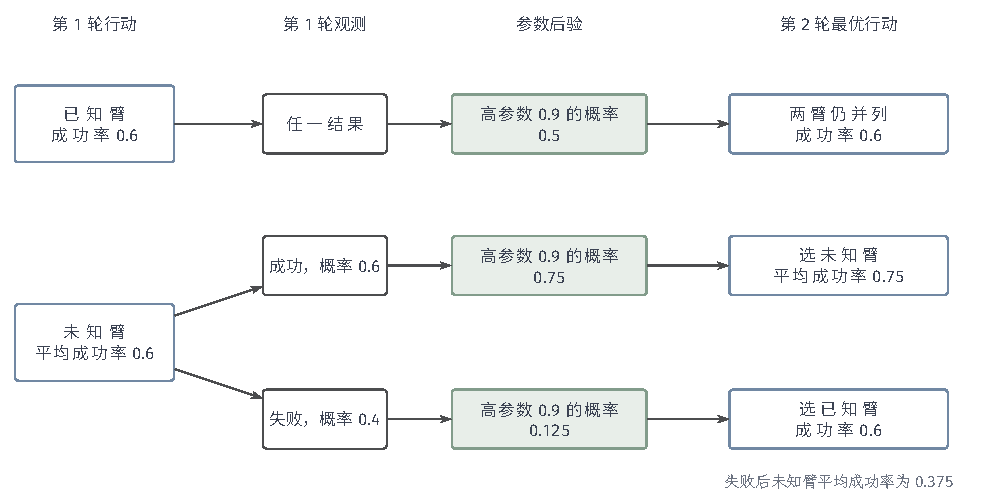
\includegraphics[width=169mm]{figures/01-mathematical-preliminaries/05-dynamical-systems-control-decision-and-games/tikz/decision-two-round-exploration/figure.pdf}
  \caption{两轮选择中的探索价值。参数\(\Theta\in\{0.3,0.9\}\)在两轮间不变，先验各为\(1/2\)；
  给定参数，各次奖励条件独立，每轮只观察所选臂。后验列给出高参数的概率，末列给出下一轮最优行动的成功率。
  先选未知臂的两轮期望为\(0.6+0.6\times0.75+0.4\times0.6=1.29\)，先选已知臂为\(1.2\)。}
  \label{fig:decision-two-round-exploration}
\end{figure*}

% v1-game-card-history-information tex/01-mathematical-preliminaries/05-dynamical-systems-control-decision-and-games/04-multi-agent-response-and-evolution.tex
\begin{figure*}[htbp]
  \centering
  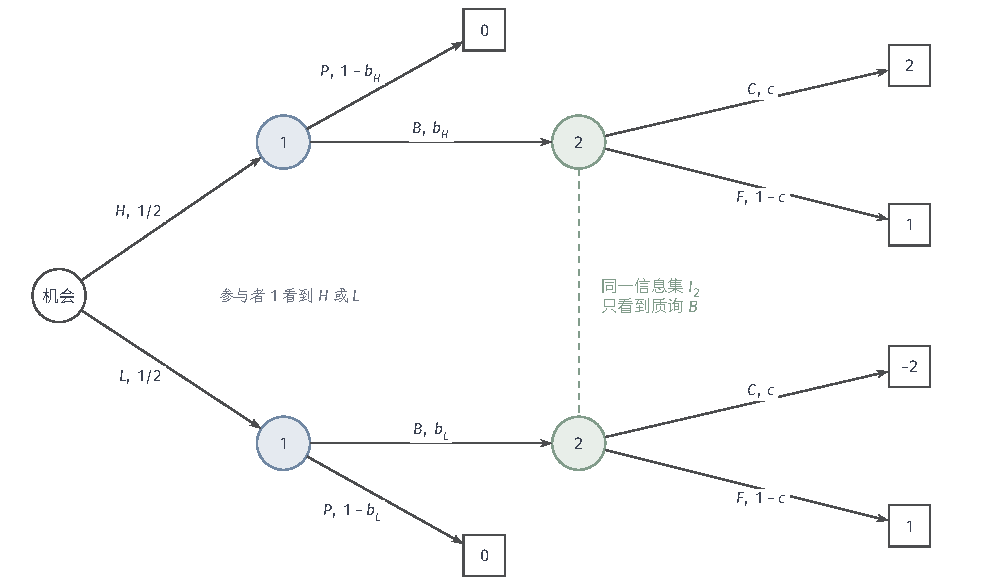
\includegraphics[width=169mm]{figures/01-mathematical-preliminaries/05-dynamical-systems-control-decision-and-games/tikz/game-card-history-information/figure.pdf}
  \caption{三张牌教学博弈的历史树。机会仅在高牌\(H\)与低牌\(L\)间等概率发牌，公共中牌\(M\)是比较基准。
  参与者1看到牌面，分别以\(b_H,b_L\)质询；参与者2只看到质询，虚线连接的信息集\(I_2\)中共用应对概率\(c\)。
  方节点标出终局收益\(u_1\)，参与者2的收益为\(-u_1\)。虚线表示无法区分的历史，不是额外行动或转移。}
  \label{fig:game-card-history-information}
\end{figure*}

% tab:rv-viewing-time-guarantees tex/01-mathematical-preliminaries/04-random-variables-distributions-and-causality/01-random-variables.tex
\begin{table*}[htbp]
  \centering\small
  \begin{tabularx}{\linewidth}{p{22mm}p{39mm}XX}
    \toprule
    查看方式 & 受控事件 & 所需保证 & 可据此判断的范围\\
    \midrule
    事先固定\(n\) & \(E_n\) & \(\mathbb P(E_n)\leq\delta\) & 只控制预先指定的这一次查看；更换成历史决定的时刻需要另行证明。\\
    最多查看\(T\)次 & \(\bigcup_{t=1}^T E_t\) & 各次\(\mathbb P(E_t)\leq\delta_t\)，且\(\sum_{t=1}^T\delta_t\leq\delta\) & 并合界控制总失败概率；事件无须相互独立。\\
    任意时刻同时有效 & \(\bigcup_{t\geq1}E_t\) & \(\mathbb P(\bigcup_{t\geq1}E_t)\leq\delta\) & 对几乎必然有限的正整数停时\(\tau\)，仍有\(\mathbb P(E_\tau)\leq\delta\)。\\
    \bottomrule
  \end{tabularx}
  \caption{查看时刻变化下的误差保证。\(E_t\)须包含所用界的完整条件：例如Freedman事件同时要求
  \(S_t\geq x\)与\(V_t\leq v\)。非负超鞅可经Ville不等式构造同时界；有界可选停止的期望等式本身不提供这类失败概率保证。}
  \label{tab:rv-viewing-time-guarantees}
\end{table*}

% tab:information-candidate-support tex/01-mathematical-preliminaries/04-random-variables-distributions-and-causality/02-information-theory-and-statistical-geometry.tex
\begin{table*}[htbp]
  \centering\small
  \begin{tabularx}{\linewidth}{XXcccc}
    \toprule
    后验\(\pi\) & 候选\(q\) & \(q\ll\pi\) & \(\pi\ll q\) & \(D_{\mathrm{KL}}(q\Vert\pi)\) & 证据恢复比例\\
    \midrule
    \((1/2,1/2)\) & \((1,0)\) & 是 & 否 & \(\log2\) & \(1/2\)\\
    \((1,0)\) & \((1/2,1/2)\) & 否 & 是 & \(+\infty\) & \(1\)\\
    \((1/2,1/2)\) & \((1/2,1/2)\) & 是 & 是 & \(0\) & \(1\)\\
    \bottomrule
  \end{tabularx}
  \caption{候选支持对KL与证据恢复的影响。两点分布共用同一取值集合，证据满足
  \(0<p_{\bm\theta}(x)<\infty\)。恢复比例为\(\mathbb E_q[p_{\bm\theta}(x,Z)/q(Z)]/p_{\bm\theta}(x)=\pi(\{q>0\})\)，
  比值仅在\(q>0\)处评价。表中的有限KL是具体例子的结果；一般空间中\(q\ll\pi\)不能单独保证KL有限。}
  \label{tab:information-candidate-support}
\end{table*}

% W1 tex/01-mathematical-preliminaries/04-random-variables-distributions-and-causality/01-random-variables.tex
\begin{aligned}
  &\int_{B_\delta(\widehat{\bm\vartheta})}
  \exp\!\left\{n\bigl[h(\bm\vartheta)
    -h(\widehat{\bm\vartheta})\bigr]\right\}
  g(\bm\vartheta)\,\mathrm d\bm\vartheta\\
  &\qquad=n^{-d/2}|\bm H|^{-1/2}
  g(\widehat{\bm\vartheta})(2\pi)^{d/2}\{1+o(1)\}.
\end{aligned}

% W2 tex/01-mathematical-preliminaries/04-random-variables-distributions-and-causality/01-random-variables.tex
\begin{aligned}
  &\int_{\Theta\setminus B_\delta(\widehat{\bm\vartheta})}
  e^{n[h(\bm\vartheta)-h(\widehat{\bm\vartheta})]}
  g(\bm\vartheta)\,\mathrm d\bm\vartheta\\
  &\qquad\leq e^{-(n-n_0)\eta}
  \int_\Theta
  e^{n_0[h(\bm\vartheta)-h(\widehat{\bm\vartheta})]}
  g(\bm\vartheta)\,\mathrm d\bm\vartheta\\
  &\qquad=o(n^{-d/2}).
\end{aligned}

% W3 tex/01-mathematical-preliminaries/04-random-variables-distributions-and-causality/01-random-variables.tex
若依概率收敛，在任意子列中递归选取指标\(n_k\)，使
\[
  \mathbb P\{d(X_{n_k},X)>2^{-k}\}\leq2^{-k}.
\]

% W4 tex/01-mathematical-preliminaries/04-random-variables-distributions-and-causality/01-random-variables.tex
积分并用Cauchy--Schwarz，得到
\[
\begin{aligned}
 \mathbb E(Y^*)^2
 &\leq2\mathbb E(|Y_N|Y^*)\\
 &\leq2\|Y_N\|_2\|Y^*\|_2,
\end{aligned}
\]
故\(\mathbb E(Y^*)^2\leq4\mathbb E Y_N^2\)。

% W5 tex/01-mathematical-preliminaries/04-random-variables-distributions-and-causality/02-information-theory-and-statistical-geometry.tex
\begin{aligned}
  \lambda\mathbb E_Q(R-\widehat R_S)
  &\leq D_{\mathrm{KL}}(Q\Vert P_0)
       +\log\mathbb E_{P_0}e^{\lambda(R-\widehat R_S)}\\
  &\leq D_{\mathrm{KL}}(Q\Vert P_0)
       +\frac{\lambda^2}{8n}+\log(1/\delta).
\end{aligned}

% W6 tex/01-mathematical-preliminaries/05-dynamical-systems-control-decision-and-games/01-action-and-state.tex
 得
 \[
  a\mathbb P(S_{\rm grid}>a)
    \leq\mathbb E[\|\bm M_T\|\mathbb I_{\{S_{\rm grid}>a\}}].
 \]

% W7 tex/01-mathematical-preliminaries/05-dynamical-systems-control-decision-and-games/01-action-and-state.tex
 \begin{aligned}
 \|\mathcal T\bm Z-\mathcal T\bm Y\|_{\mathcal S^2}^2
 &\leq(2hL^2+8L^2)\int_a^{a+h}
                   \mathbb E\|\bm Z_s-\bm Y_s\|^2\,\mathrm ds\\
 &\leq2L^2h(h+4)\|\bm Z-\bm Y\|_{\mathcal S^2}^2.
 \end{aligned}

% Final new lead paragraphs, each read continuously with its preceding definition and following figure/table.
% N10-P1 tex/01-mathematical-preliminaries/04-random-variables-distributions-and-causality/01-random-variables.tex
用同一族失败事件\(E_t\)表示第\(t\)次查看时所用误差界被违反。表~\ref{tab:rv-viewing-time-guarantees}
比较时间量词：采用并合界合并逐次保证时，需要为各次查看分配失败概率。

% N11-P1 tex/01-mathematical-preliminaries/04-random-variables-distributions-and-causality/02-information-theory-and-statistical-geometry.tex
表~\ref{tab:information-candidate-support}将支持方向与两种计算并列。完整恢复证据要求候选覆盖后验，
而有限的\(D_{\mathrm{KL}}(q\Vert\pi)\)还要求候选不在零后验区域放置质量；两者控制的对象不同。

% N15-P1 tex/01-mathematical-preliminaries/05-dynamical-systems-control-decision-and-games/03-policy-value-and-optimization.tex
图~\ref{fig:decision-two-round-exploration}把这两条选择路径展开。第一轮的平均收益相同，
但未知臂的结果改变参数后验，从而改变第二轮的最优行动。

% N16-P1 tex/01-mathematical-preliminaries/05-dynamical-systems-control-decision-and-games/04-multi-agent-response-and-evolution.tex
图~\ref{fig:game-card-history-information}保留两条质询历史，并以同一信息集连接参与者2的决策节点。
两处行动概率相同来自信息约束，不能随隐藏牌面分别设定。
